\chapter{LA REPRESENTATION DE LA DONNEE}

\section{Introduction}
     \vspace{1em}

Envoyer une donnée sur un réseau n’est pas aussi simple que l’on croit.
     \vspace{1em}

 \begin{wrapfigure}{r}{3cm}
\Youtube{https://youtu.be/k-RhgiwKx2M}
\end{wrapfigure}
Il faut faire la différence entre le format utilisé pour stocker des données dans la mémoire de l'ordinateur et celui employé pour l'envoyer à une autre machine. En effet, chaque machine à sa propre représentation souvent liée aux capacités de leur processeur. Cela est surtout vrai pour les nombres. Ils peuvent être stockés sur un nombre de bits plus ou moins important ou peuvent être représentés en mémoire de manière optimisée pour accélérer leur traitement. 

En revanche, la représentation des chaînes de caractères (non accentués) est relativement uniforme car elle se base sur le code ASCII qui est le même pour tous les ordinateurs. Un texte de base est facilement compréhensible par toutes les machines. Une solution serait donc de n'utiliser que des chaînes de caractères. 

     \vspace{1em}

Par exemple, si l’on veut envoyer l'entier ayant pour valeur 123, il existe plusieurs représentations possibles :
\begin{itemize}
\item envoyer une chaîne de caractères ”123” contenant les chiffres du nombre ;
\item envoyer la valeur binaire 1111011.
\end{itemize}

     \vspace{1em}

On voit que juste pour transmettre une simple valeur stockée dans la mémoire d'un ordinateur, il existe plusieurs options et évidemment pour que cette valeur soit interprétée de la bonne façon, il faut que les deux extrémités se soient mises d'accord sur une représentation.

Quand on veut transmettre plusieurs valeurs, c'est-à-dire quand on a des données structurées, d'autres problèmes surviennent.

Par exemple : quelle est la taille des blocs que l’on va transmettre ? Comment indiquer la fin de la transmission ? Pour une chaîne de caractères, comment indiquer qu’elle se termine ? Autre exemple : si l'on veut transmettre "12" puis "3", comment faire pour que l'autre extrémité ne comprenne pas "123" ?

     \vspace{1em}


Pour que la transmission se fasse correctement, il faut que l’émetteur et le récepteur adoptent les mêmes conventions. Quand il s’agit d’un ensemble de données, il faut être capable de les séparer. Avec les tableurs, une première méthode est possible avec la notation \ac{CSV} Comme son nom l’indique, les valeurs sont séparées par des virgules. Les valeurs sont représentées par des chaînes de caractères. Les textes sont différenciés des valeurs numériques, par l’utilisation de guillemets. Ainsi, 123 sera interprété comme un nombre et ”123” comme un texte.

Si cette représentation est adaptée aux tableurs, elle est relativement pauvre car elle ne permet de représenter que des valeurs sur des lignes et des colonnes. Pour les usages du Web, il a fallu trouver un format plus souple permettant de représenter des structures de données complexes. Évidemment, comme rien n'est simple, il en existe plusieurs et les applications échangeant des données devront utiliser le même.

     \vspace{1em}


On voit que l'envoi de la chaîne de caractères ne suffit pas, il faut la formater pour que le récepteur puisse trouver le type de la donnée transmise, qu'un nombre ne soit pas interprété comme une chaîne de caractères, qu'une chaîne de caractères reste une chaîne de caractères même si elle ne contient que des chiffres.   
    \vspace{1em}
   
\section{La \Index{sérialisation}}

Sous ce nom barbare se cache la méthode utilisée pour transmettre 
des données d’un ordinateur à un autre.
Une donnée peut être simple
(un nombre, un texte) ou plus complexe (un tableau, une structure...). 
Elle est stockée dans la mémoire de l'ordinateur suivant une représentation qui lui est propre. Par exemple, la taille des entiers peut varier d'une technologie de processeur à une autre, l'ordre des octets dans un nombre peut aussi être différente (little et big endian). 
Pour des structures complexes comme les tableaux, les éléments peuvent être rangés à différents emplacements de la mémoire. 

La sérialisation consiste à transformer une structure de données en une séquence qui pourra être transmise sur le réseau, stockée dans un fichier ou une base de données. L'opération inverse, consistant à reconstruire localement une structure de données, s'appelle désérialisation. 

Il existe plusieurs formats pour sérialiser les données. Ils peuvent être binaires mais ceux généralement utilisés sont basés sur des chaînes de caractères. En effet, la représentation \ac{ASCII} définissant les caractères de base et codée sur 7 bits est commune à l'ensemble des ordinateurs. L'autre avantage du code ASCII est qu'il est facilement lisible et simplifie la mise au point des programmes.  

Wikipédia donne ce tableau (cf. figure~\vref{fig-ASCII}) des codes \ac{ASCII} datant de 1972 (une éternité en informatique) et recolorisé par nos soins.

\begin{figure}[tbp]
\centerline{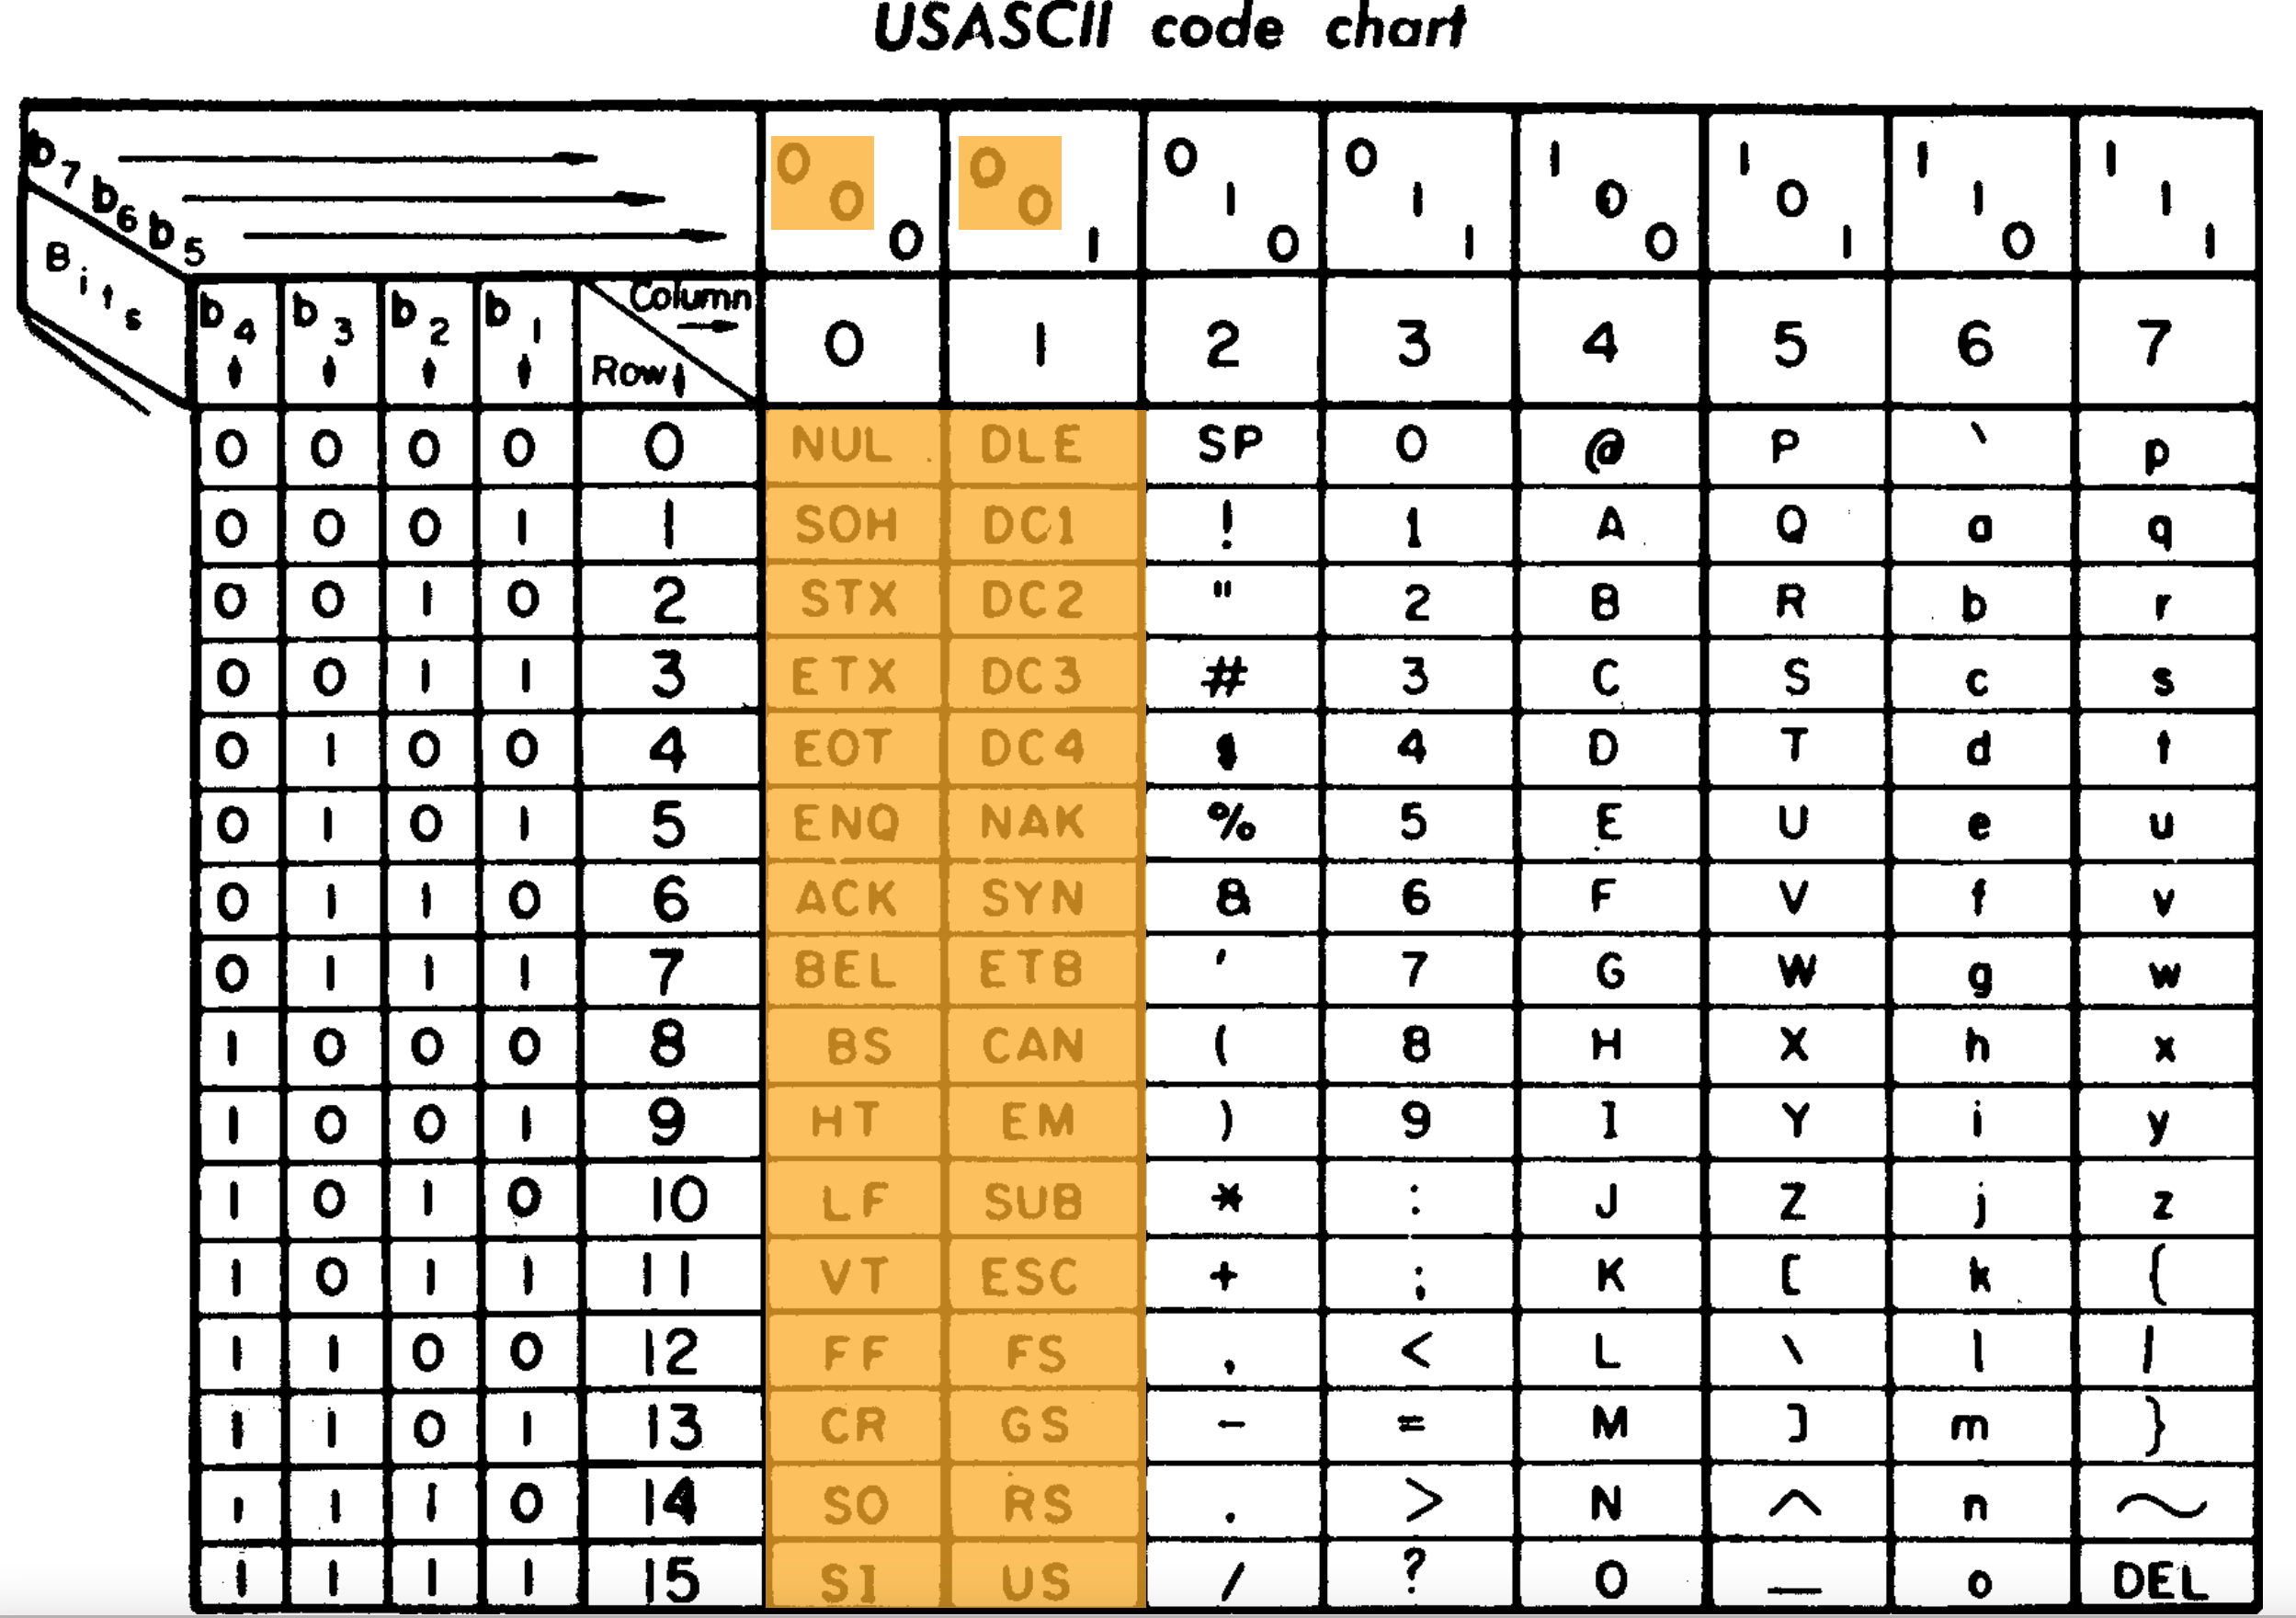
\includegraphics[width=1\columnwidth]{Pictures/Capture20.png}}
\caption{Codage ASCII des caractères}
\label{fig-ASCII}
\end{figure}

Les caractères en orange ne sont pas imprimables. Ils permettent de contrôler la communication des données ou de gérer l'affichage en revenant à la ligne. On les reconnait car la séquence binaire commence par 00X XXXX. On rappelle que le code ASCII est sur 7 bits ; le bit supplémentaire (bit de parité) conduisant à 1 octet était utilisé pour détecter des erreurs de transmission. Les valeurs de 0x30 à 0x39 codent les chiffres de 0 à 9. 

\subsection*{Hexlify}

En Python, il existe le module \Index{binascii} très pratique qui permet de convertir une séquence binaire en une chaîne de caractères ou inversement :
\begin{itemize}
\item \pfunction{binascii}{hexlify} prend un tableau d'octets et le convertit en une chaîne de caractères hexadécimaux plus lisible pour les spécialistes. Cela permet de visualiser n'importe quelle séquence de données. 
\item \pfunction{binascii}{unhexify} fait l'inverse. Il prend une chaîne de caractères et la convertit en un tableau d'octets. Cela peut vous faciliter la programmation car, dans votre code, il est plus facile de manipuler des chaînes de caractères.

\end{itemize}
Dans la suite, nous l'utiliserons pour manipuler des identifiants. Par exemple, ce bout de code illustre l'utilisation de ces fonctions :

\begin{python}
mac = lora.mac()
print ('devEUI: ',  binascii.hexlify(mac))

# create an OTAA authentication parameters
app_eui = binascii.unhexlify('70 B3 D5 7E D0 03 3A E3'.replace(' ',''))

\end{python}

Comme nous le verrons par la suite, a fonction \pfunction{network}{lora.mac()} retourne un tableau d'octets. La fonction \pfunction{binascii}{hexlify} ligne suivante le convertit en chaîne de caractères pour un affichage plus propre. 

Inversement, nous devons affecter une séquence binaire à la variable \texttt{app\_eui}. Nous mettons cette séquence hexadécimale en chaîne de caractères. Les espaces offrent plus de lisibilité. Ils sont retirés par la méthode replace et le résultat est converti en binaire grâce à \pfunction{binascii}{unhexify}

\section{Base64}

Le passage d'une séquence binaire à une chaîne de caractères ASCII en représentant les valeurs conduit à un doublement du volume. Chaque bloc de 4 bits va conduire à produire un octet correspondant au caractère d'un chiffre ou d'une lettre de A à F. Le reste des codes n'est pas utilisé.

Le codage base64 offre un meilleur rendement en utilisant 64 bits pour coder les valeurs. Un dictionnaire fait la correspondance entre 64 valeurs et un caractère ASCII. Cependant, si l'on veut coder 4 octets, soit 32 bits, il faudra 5 blocs de 6 bits, et il y aura deux bits restants. Le symbole = indique que 2 bits sont ajoutés à la fin du codage. Donc, dans notre cas, il faudra ajouter deux symboles = comme le montre la figure ci-dessous :

\begin{figure}[tbp]
\centerline{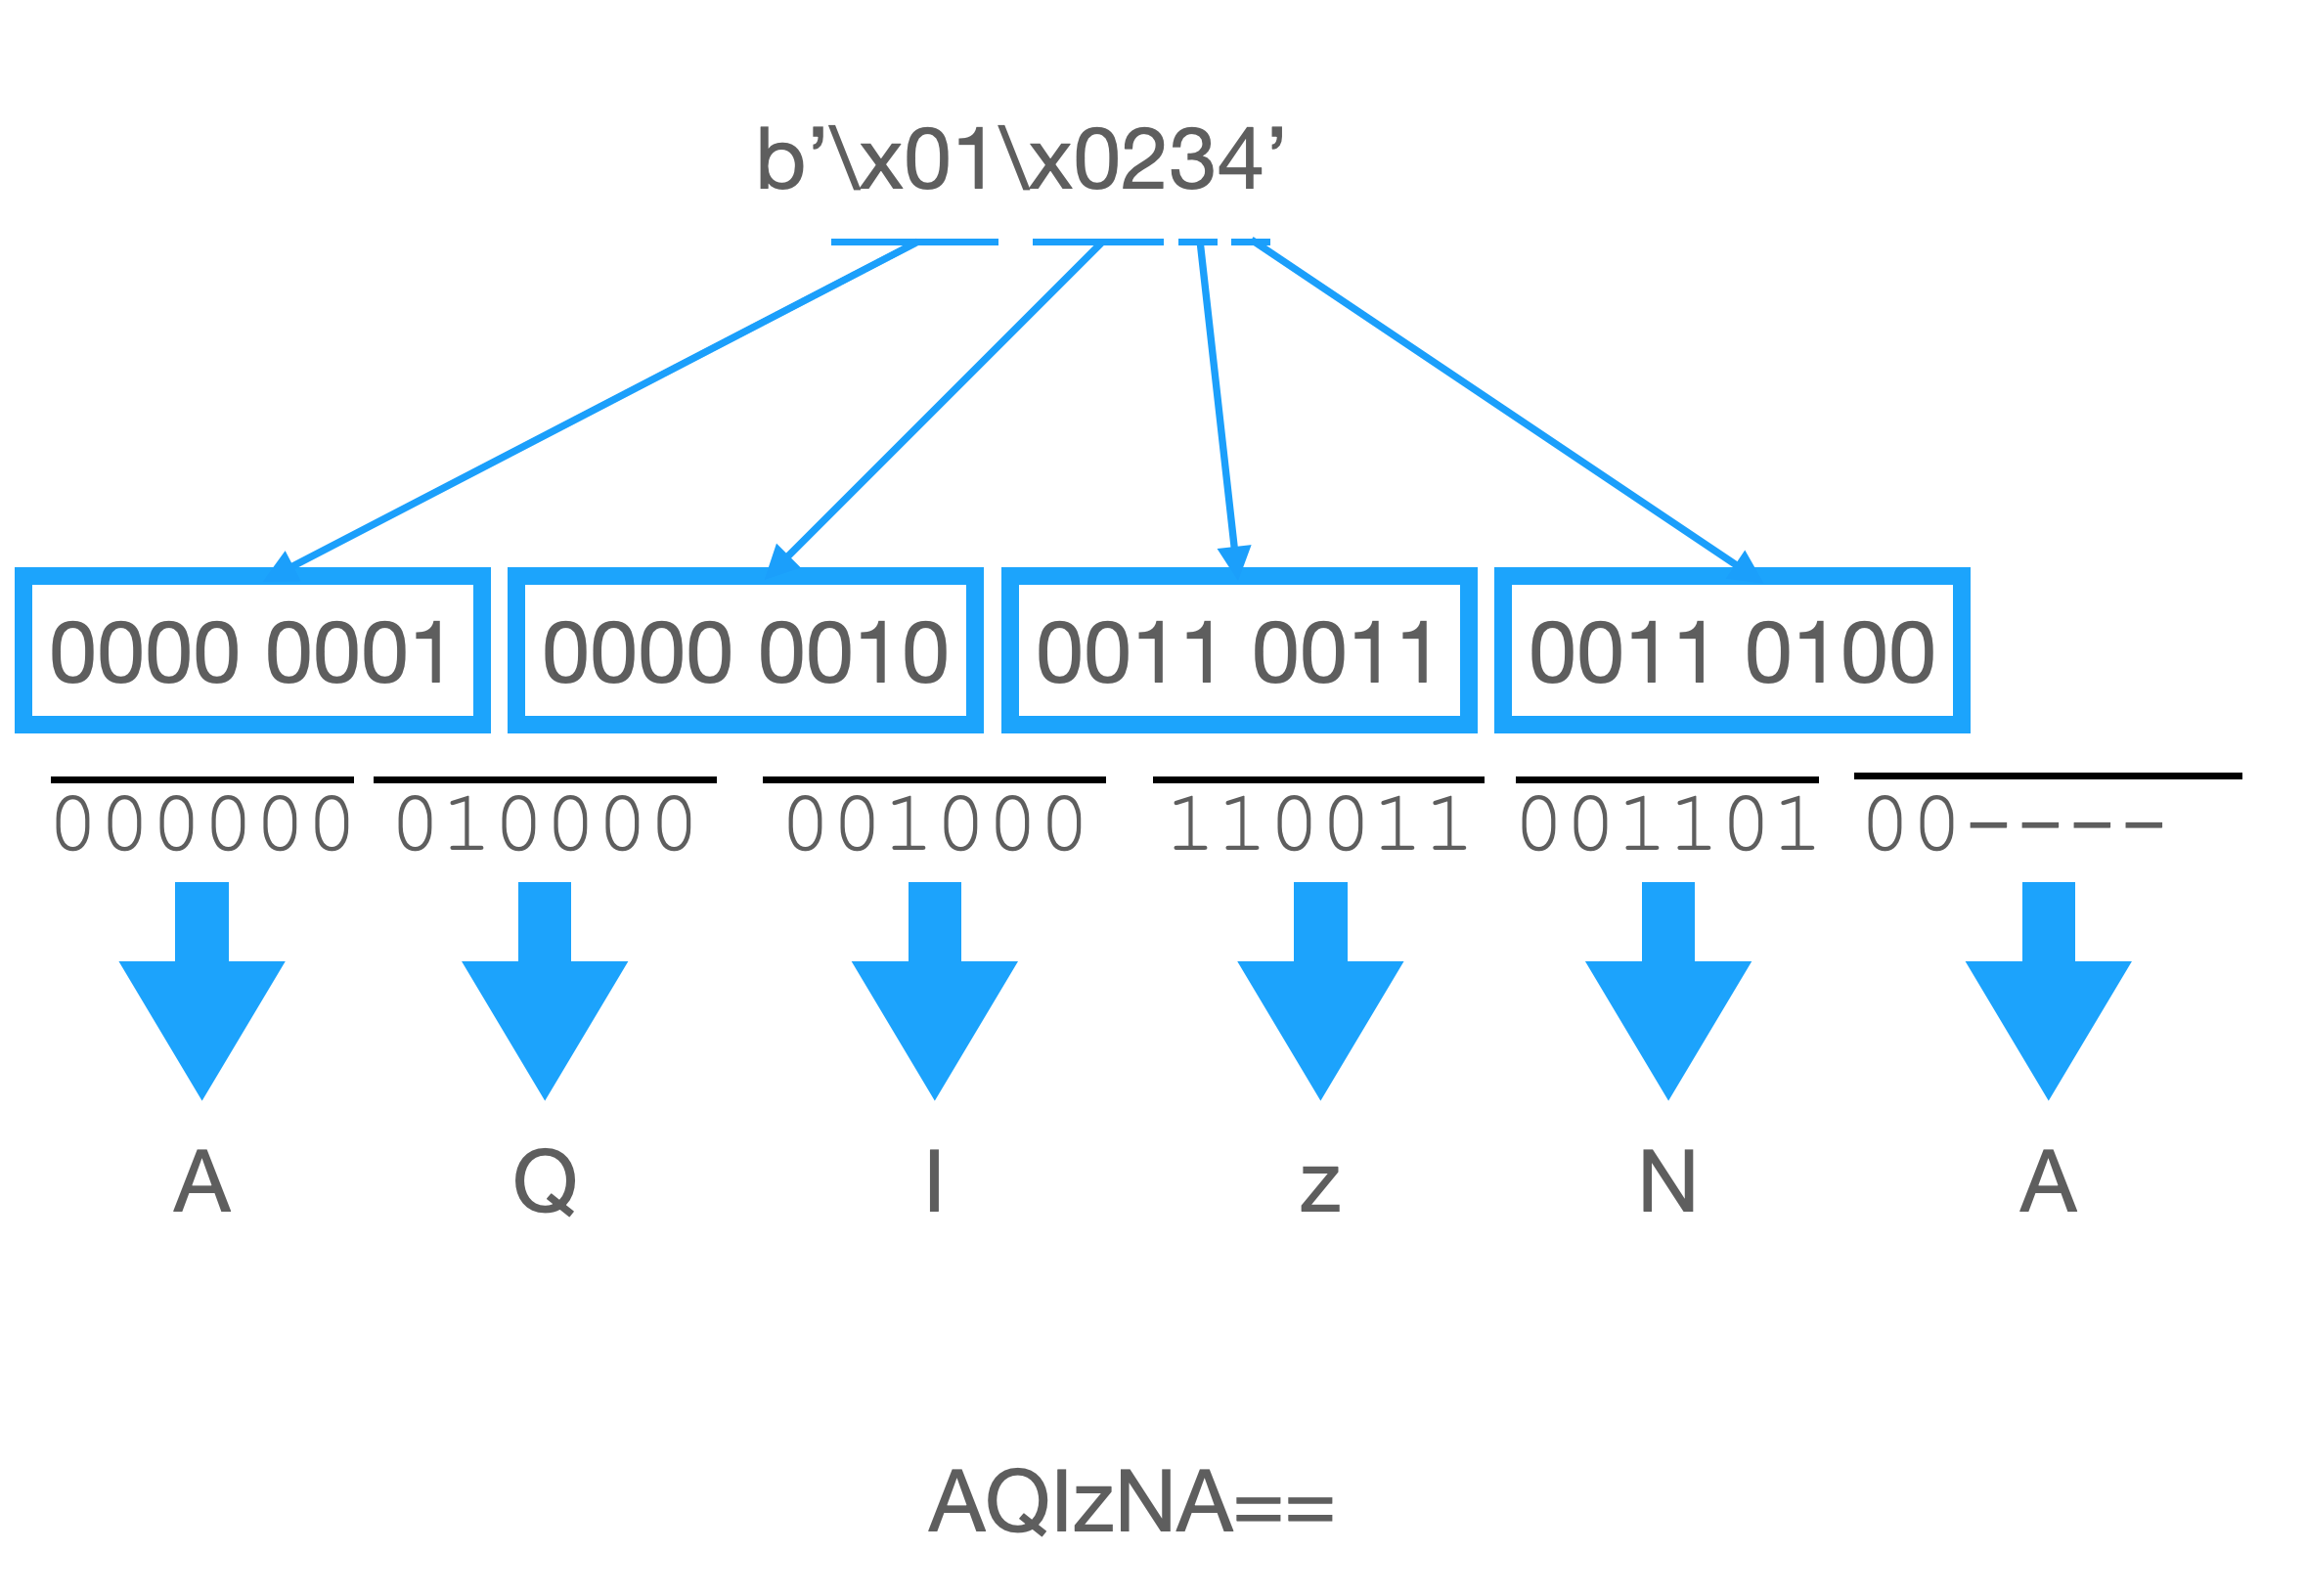
\includegraphics[width=1\columnwidth]{Pictures/Capture21.png}}
\caption{Codage Base64 de données binaires}
\label{fig-base64}
\end{figure}

On notera que pour les petites séquences, ce codage n'est pas meilleur que la transformation de la séquence hexadécimale en chaîne de caractères. Ici, il faut 8 caractères pour coder 4 octets. 

Il existe beaucoup d'outils en ligne pour faire les conversions entre ces différentes représentations, comme le site \url{www.asciitohex.com}.

\subsection*{Python module: base64}

En Python3, le module base64 permet de faire ces conversions.  Ce module est un peu susceptible sur les types de données à utiliser.

\begin{python}[numbers=left,numbersep=5pt]
import base64

val = b"\x01\x0234"
ser = base64.b64encode(val)
print (ser)
print (ser.decode())
ori = base64.b64decode(ser)
print (ori)
\end{python}

qui donne à l’exécution :

\begin{termc}[backgroundcolor=\color{backcolour}]
b'AQIzNA=='
AQIzNA==
b'\x01\x0234'
\end{termc}

À noter que l'utilisation du \texttt{ser.\pfunction{str}{decode()}}, ligne 6, pour transformer une chaîne d'octets en chaîne de caractères, c'est-à-dire supprimer le \texttt{b} du début, peut être utilisé dans certains cas.



\section{HTML}

La sérialisation en chaînes de caractères (par exemple en Python via la commande \pfunction{binascii}{hexlify}) ou en Base64 concerne surtout des données binaires. Mais la donnée peut être aussi structurée, par exemple la page d'un tableur. Il faut donc formater le document pour éviter une fusion des différents champs.


\ac{HTML}, sans entrer dans les détails, définit un format où les champs sont repérés par un balisage.  Une balise de début est un mot clé entre \texttt{<>} et, pour une \Index{balise} de fin, le mot clé est précédé du caractère \texttt{/}. Par exemple, la figure~\vref{fig-HTML} avec le balisage, le premier paragraphe est formaté de cette manière, Dans le MOOC :

\begin{figure}[tbp]
\centerline{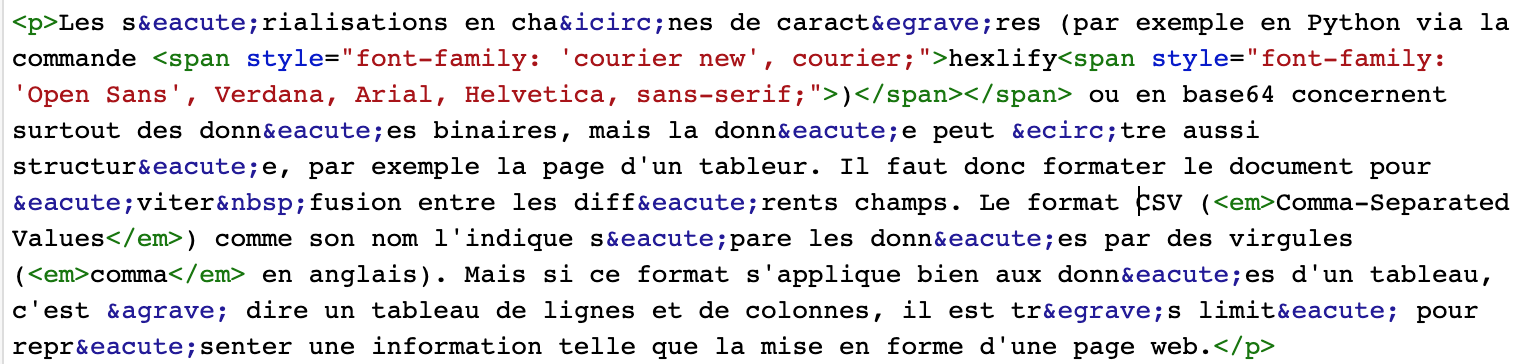
\includegraphics[width=1\columnwidth]{Pictures/Capture22.png}}
\caption{Codage HTML d'une page Web}
\label{fig-HTML}
\end{figure}

Les balises peuvent aussi prendre des arguments, comme la balise \Index{span} dans l'exemple précédent. Ainsi, si l'on regarde une page Web, comme indiqué figure~\vref{fig-Web-HTML}, le navigateur est capable de l'analyser pour trouver les \ac{URI} qu'elle contient. La balise \texttt{\Index{img}} indiquant qu'il s'agit d'une image, le client peut interroger le serveur pour l'afficher à l'écran. Ce format structuré de sérialisation nous permet de mettre en place une caractéristique de \ac{REST}, c'est-à-dire les liens entre ressources.

\begin{figure}[tbp]
\centerline{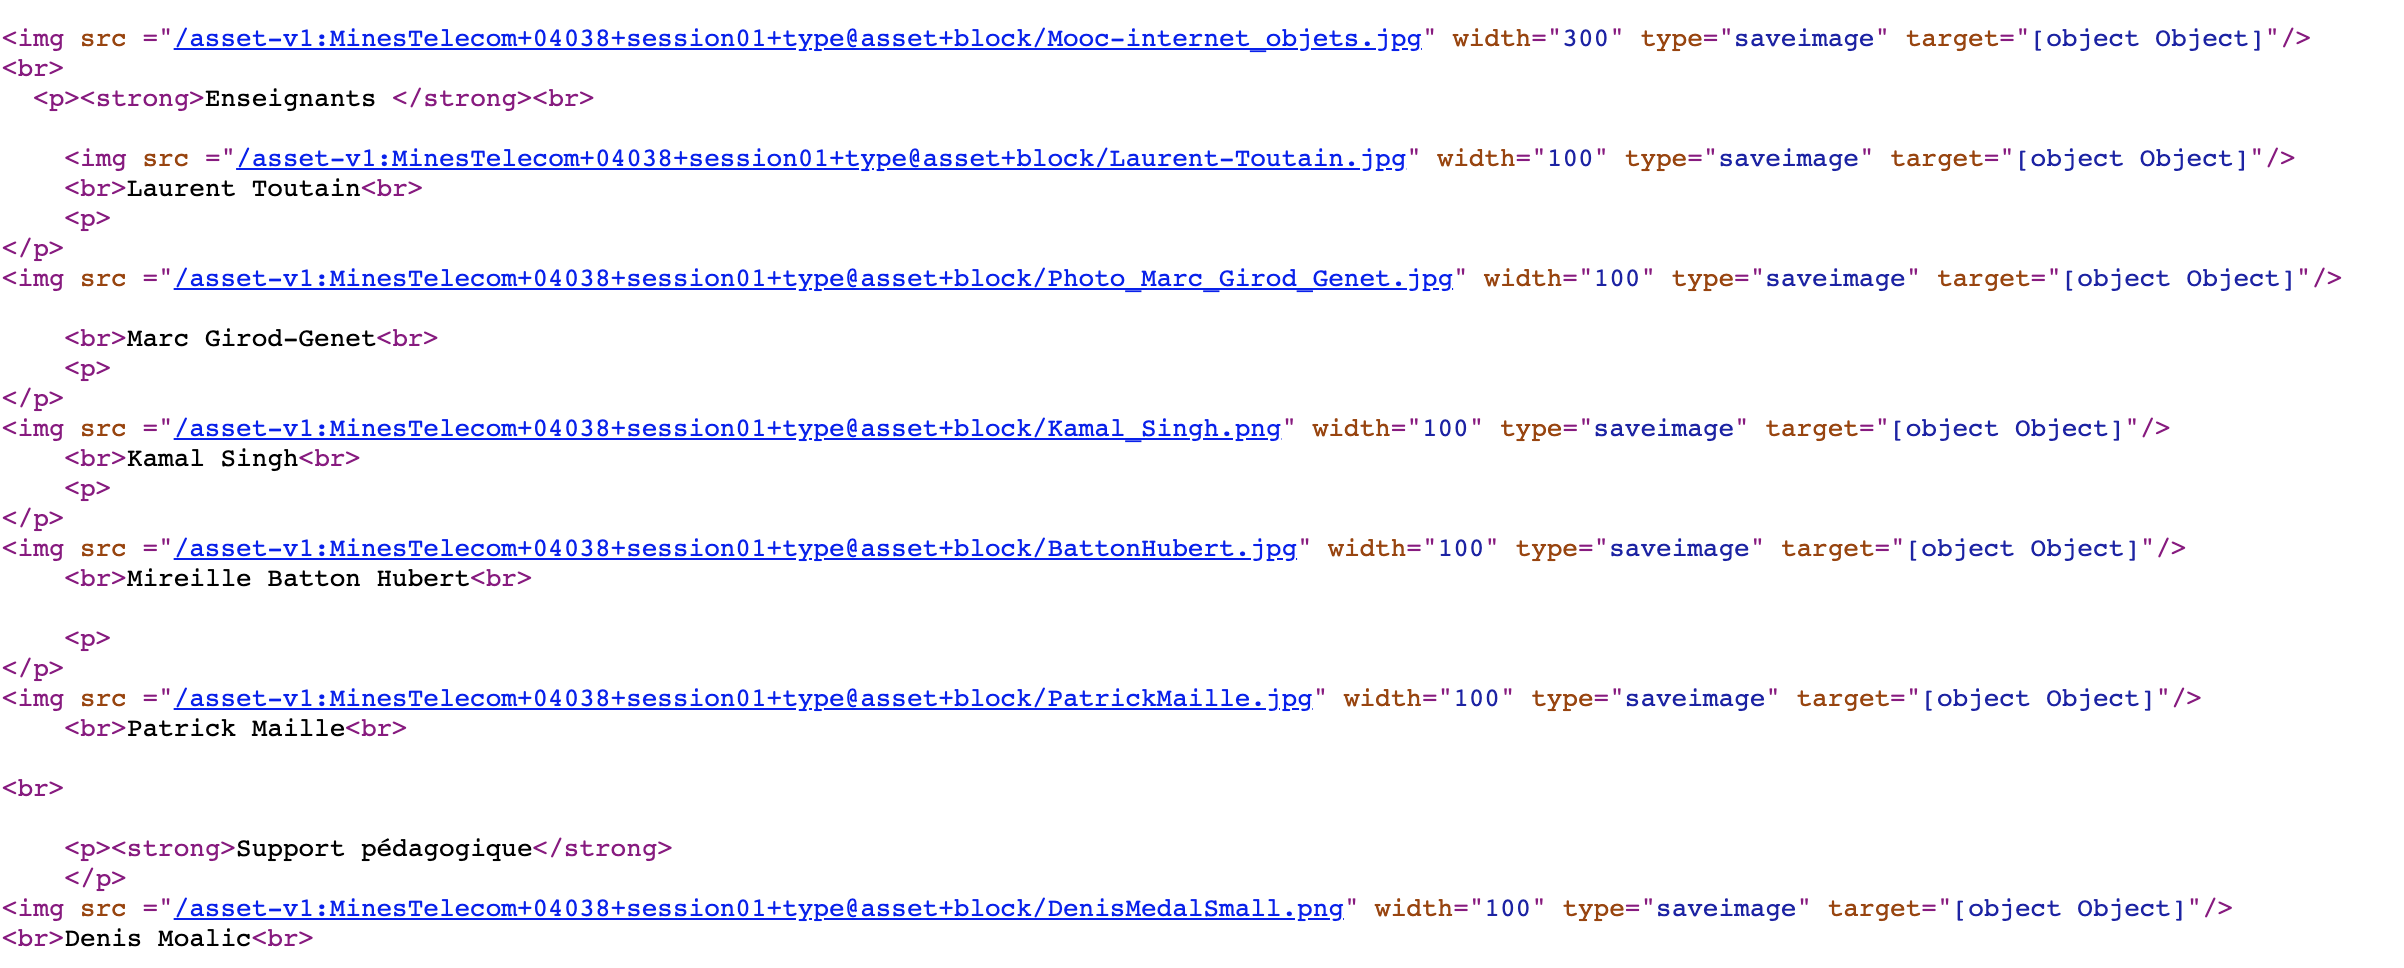
\includegraphics[width=1\columnwidth]{Pictures/Capture23.png}}
\caption{Capture d'une page Web}
\label{fig-Web-HTML}
\end{figure}


\section{XML}

Si \ac{HTML} est dédié au formatage à l'écran de données textuelles et à la navigation sur le Web. \ac{XML}\footnote{\url{https://www.w3.org/TR/xml/}} défini par le \ac{W3C}, est un format d’échange entre deux applications. Par exemple, pour échanger les notes des étudiants entre la plate-forme FUN et une autorité de certification des cours, on pourrait utiliser le format suivant~:

\begin{termc}[backgroundcolor=\color{gray!10}]
<etudiant>
   <prenom>John</prenom>
   <nom>Deuf</nom>
   <note>18</note>
</etudiant>

\end{termc}

Il est facile en lisant l'exemple de trouver le prénom, le nom et la note de l'étudiant. On peut noter qu'il n'y a pas de différence entre la note et le nom de l'élève. Il s'agit de caractères.

     \vspace{1em}

S'il est syntaxiquement correct, rien ne dit que le créateur fournit quelque chose de correct qui pourra être interprété par une autre instance.  \ac{XML} peut inclure une grammaire ou un schéma qui est utilisé pour valider que les informations représentées dans le fichier sont non seulement syntaxiquement conformes au langage \ac{XML}, mais aussi conformes au schéma. Ce schéma va décrire les champs attendus et leur type (texte, nombre...). Vous pouvez accéder à ce cours si vous voulez en savoir plus sur les schémas \ac{XML}.

Du point de vue de l’internet des objets, même si le XML pourrait être un bon candidat pour l’échange d’informations, il est un format trop lourd et donc énergivore. On peut noter que pour envoyer une note sur 20 qui, dans l'absolu, prendrait 6 bits, on transmet \texttt{<note>18</note>}, soit 15 caractères soit 120 bits! 

\section{JSON}

 \begin{wrapfigure}{r}{3cm}
\Youtube{https://youtu.be/IhZ9w6jWnq8}
\end{wrapfigure}

\ac{JSON}  offre un moyen de structurer l’information de manière plus compacte que \ac{XML}. JSON s’impose comme le langage commun pour échanger les informations. A l’origine, JSON était utilisé par\Index{Javascriptt} pour échanger des informations ; par exemple, pour afficher en temps réel l’évolution des cours de la bourse ou pour afficher des graphiques dynamiques sur l’écran de l’utilisateur.

JSON \rfc{8259} est un format d’échange simple. Il définit 4 types de données :

\begin{itemize}
    \item nombre~: Les nombres sont composés de chiffres et peuvent être positifs, négatifs, entiers ou flottants.
    \item texte~: Le texte est délimité par des guillemets simples ou doubles.
    \item \Index{tableau}~: Les tableaux sont des listes d’éléments séparés par des virgules et entourés de crochets.
    \item \Index{objet}~: L’objet est une liste de paires composées d’une \Index{clé} et d’une valeur. La clé est une chaîne de caractères et la valeur peut être de n’importe quel type. La clé doit être unique à l’intérieur d’un objet, et référence entièrement la valeur qui la suit. Le couple clé - valeur est séparé par le caractère 2 points  \texttt{:}. Les éléments de l’objet sont séparés par des virgules. L'objet est délimité par des accolades.
\end{itemize}

Par exemple, quelques structures \ac{JSON} :

\begin{itemize}
    \item \texttt{[1, -2, 0.3, 4e1]} est un tableau qui contient 4 nombres ;
    \item \texttt{[1, ”2”, ”34”]} est un tableau contenant un nombre et deux chaines de caractères ;
    \item \texttt{[1, [2, 3 , ”4”]]} est un tableau de deux éléments dont le second est également un tableau de 3 éléments ;
    \item \texttt{\{ ”couleur” : [34, 16, 3]\}} est un objet qui contient un élément et la valeur est un tableau ; 
    \item \texttt{\{ ”name” : ”bob”, ”age” : 30\}} est un objet qui contient deux éléments référencés par les chaînes de caractères (ou index)  ”name” et ”age”.
    
    L’ordre dans lequel sont placés les éléments est indifférent. \texttt{\{”age” : 30, ”name” : ”bob”\}} est équivalent au dernier exemple. 

    Cela impose que l’index utilisé pour accéder à une valeur doit être unique dans la structure objet \texttt{\{”name” : ”bob”, ”name” : ”alice”}\} est interdit.
\end{itemize}

     \vspace{1em}

Le listing suivant donne un exemple de structure JSON tirée du \rfc{8259}. Il contient un objet JSON avec une seule clé \texttt{”Image”}. La valeur de cette clé est une autre structure qui contient six éléments. 

\begin{termc}[backgroundcolor=\color{gray!10}, language=json]
{
"Image": {
      "Width": 800,
      "Height": 600,
      "Title": "View from 15th Floor",
      "Thumbnail": {   
           "Url": "http://www.example.com/image/481989943",
           "Height": 125,
           "Width": 100
       },
       "Animated" : false,
       "IDs": [11, 943, 234, 38793]
    }
}
\end{termc}

Le balisage par clé est un élément fondamental dans la structure des données. Il est primordial d'être cohérent et d'assurer une concordance entre émetteur et récepteur sur l'intitulé de la clé pour pouvoir récupérer l'information voulue. De la même façon, il faut s'accorder sur les unités de mesure : une interprétation d'une mesure en centimètre alors qu'elle est en pixel peut être désastreux ; c'est un problème d'interopérabilité.
     \vspace{1em}

JSON est facilement exploitable dans d’autres langages. Par exemple en Python, le module JSON peut être utilisé pour convertir une structure JSON qui est une chaîne ASCII en une représentation interne Python. Les tableaux sont convertis en listes et les objets en dictionnaires.

     \vspace{1em}
     \pythonlst{example\_json.py}

Le programme \pprog{example\_json.py} reprend la structure précédente. La variable \texttt{struct\_python} est une structure Python. On peut voir que les valeurs pour \texttt{"Animated"} et \texttt{"Copyright"} sont les mots clé Python \texttt{False} (avec un F majuscule) et \texttt{None}. Le programme affiche deux fois cette valeur avec la commande standard \texttt{print} puis avec le module \pfunction{pprint}{pprint} pour avoir un affichage plus lisible. On peut remarquer que l'ordre d'affichage des clés est différent. Comme \texttt{"Title"} était défini deux fois, seul le dernier est conservé dans la structure Python.

\begin{termc}[backgroundcolor=\color{gray!10}, language=json, basicstyle=\tiny]
{'Image': {'IDs': [17, 2371, 234, 38793], 'Height': 600, 'Animated': False, 'Title': 'Empty picture', 'Thumbnail': 
{'Url': 'http://www.example.com/image/481989943', 'Width': 100, 'Height': 125}, 'Width': 800, 'Copyright': None}}
{'Image': {'Animated': False,
           'Copyright': None,
           'Height': 600,
           'IDs': [17, 2371, 234, 38793],
           'Thumbnail': {'Height': 125,
                         'Url': 'http://www.example.com/image/481989943',
                         'Width': 100},
           'Title': 'Empty picture',
           'Width': 800}}
\end{termc}

Grâce à la fonction \pfunction{json}{dumps} du module \texttt{json}, la variable \texttt{struct\_python} est transformée en JSON. Les mots clé  \texttt{False} et  \texttt{None} sont remplacés par  \texttt{false} et  \texttt{null}. Le programme affiche une chaîne de caractères.

\begin{termc}[backgroundcolor=\color{gray!10}, language=json, basicstyle=\tiny]
{"Image": {"IDs": [17, 2371, 234, 38793], "Height": 600, "Animated": false, "Title": "Empty picture", "Thumbnail": 
{"Url": "http://www.example.com/image/481989943", "Width": 100, "Height": 125}, "Width": 800, "Copyright": null}}
\end{termc}

Pour le retransformer, de JSON en variable Python, on utilise la fonction inverse \pfunction{json}{loads} qui traduit une chaîne de caractères en variable Python.

\begin{termc}[backgroundcolor=\color{gray!10}, language=json, basicstyle=\tiny]
{'Image': {'Animated': False,
           'Copyright': None,
           'Height': 600,
           'IDs': [17, 2371, 234, 38793],
           'Thumbnail': {'Height': 125,
                         'Url': 'http://www.example.com/image/481989943',
                         'Width': 100},
           'Title': 'Empty picture',
           'Width': 800}}
\end{termc}


Les autres langues de programmation possèdent également leur propre bibliothèque pour effectuer la traduction.

     \vspace{1em}

Par rapport à \ac{XML}, \ac{JSON} est beaucoup plus permissif et manque de formalisme pour décrire la structure. \ac{JSON-LD} défini par le \ac{W3C} renforce l’interopérabilité de JSON en introduisant des clés spécifiques décrivant la structure des données, une référence aux unités, etc. Nous verrons ces concepts dans la suite du cours.

\section{CBOR}

\begin{wrapfigure}{r}{3cm}
\Youtube{https://youtu.be/thSWuJ-1ld0}
\end{wrapfigure}
